% THIS IS SIGPROC-SP.TEX - VERSION 3.0
% WORKS WITH V3.1SP OF ACM_PROC_ARTICLE-SP.CLS
% JUNE 2007
%
% It is an example file showing how to use the 'acm_proc_article-sp.cls' V3.1SP
% LaTeX2e document class file for Conference Proceedings submissions.
% ----------------------------------------------------------------------------------------------------------------
% This .tex file (and associated .cls V3.1SP) *DOES NOT* produce:
%       1) The Permission Statement
%       2) The Conference (location) Info information
%       3) The Copyright Line with ACM data
%       4) Page numbering
% ---------------------------------------------------------------------------------------------------------------
% It is an example which *does* use the .bib file (from which the .bbl file
% is produced).
% REMEMBER HOWEVER: After having produced the .bbl file,
% and prior to final submission,
% you need to 'insert'  your .bbl file into your source .tex file so as to provide
% ONE 'self-contained' source file.
%
% Questions regarding SIGS should be to
% Adrienne Griscti ---> griscti@acm.org
%
% Questions/suggestions regarding the guidelines, .tex and .cls files, etc. to
% Gerald Murray ---> murray@acm.org
%
% For tracking purposes - this is V3.0SP - JUNE 2007

\documentclass{sig-alternate}

\include{macros}

\begin{document}

\conferenceinfo{ESEC-FSE'09,} {August 23--28, 2009, Amsterdam, The Netherlands.} 
\CopyrightYear{2009}
\crdata{978-1-60558-001-2/09/08} 

\title{MSeqGen: Object-Oriented Unit-Test Generation via Mining Source Code\titlenote{This work is supported in part by NSF grant CCF-0725190 and Army Research Office grant W911NF-08-1-0443.}}
%
% You need the command \numberofauthors to handle the 'placement
% and alignment' of the authors beneath the title.
%
% For aesthetic reasons, we recommend 'three authors at a time'
% i.e. three 'name/affiliation blocks' be placed beneath the title.
%
% NOTE: You are NOT restricted in how many 'rows' of
% "name/affiliations" may appear. We just ask that you restrict
% the number of 'columns' to three.
%
% Because of the available 'opening page real-estate'
% we ask you to refrain from putting more than six authors
% (two rows with three columns) beneath the article title.
% More than six makes the first-page appear very cluttered indeed.
%
% Use the \alignauthor commands to handle the names
% and affiliations for an 'aesthetic maximum' of six authors.
% Add names, affiliations, addresses for
% the seventh etc. author(s) as the argument for the
% \additionalauthors command.
% These 'additional authors' will be output/set for you
% without further effort on your part as the last section in
% the body of your article BEFORE References or any Appendices.

\numberofauthors{1} %  in this sample file, there are a *total*
% of EIGHT authors. SIX appear on the 'first-page' (for formatting
% reasons) and the remaining two appear in the \additionalauthors section.
%

\author{Suresh Thummalapenta$^1$, Tao Xie$^1$, Nikolai Tillmann$^2$, Jonathan de Halleux$^2$, Wolfram Schulte$^2$\\
\small{$^1$Department of Computer Science, North Carolina State University, Raleigh}\\
\small{$^2$Microsoft Research, One Microsoft Way, Redmond}\\
\small{$^1$\{sthumma, txie\}@ncsu.edu, $^2$\{nikolait, jhalleux, schulte\}@microsoft.com}\\
}

%\author{
% You can go ahead and credit any number of authors here,
% e.g. one 'row of three' or two rows (consisting of one row of three
% and a second row of one, two or three).
%
% The command \alignauthor (no curly braces needed) should
% precede each author name, affiliation/snail-mail address and
% e-mail address. Additionally, tag each line of
% affiliation/address with \affaddr, and tag the
% e-mail address with \email.
%
% 1st. author
%\alignauthor
%Suresh Thummalapenta\\
%       \affaddr{Department of Computer Science}\\
%       \affaddr{North Carolina State University}\\
%       \affaddr{Raleigh, USA}\\
%       \email{sthumma@ncsu.edu}
%% 2nd. author
%\alignauthor
%Tao Xie\\
%			 \affaddr{Department of Computer Science}\\
%       \affaddr{North Carolina State University}\\
%       \affaddr{Raleigh, USA}\\
%       \email{xie@csc.ncsu.edu}% 3rd. author
%\and
%\alignauthor Nikolai Tillmann, Jonathan de Halleux, Wolfram Schulte\\
%       \affaddr{Microsoft Research}\\
%       \affaddr{One Microsoft Way, Redmond, USA}\\
%       \email{\{nikolait, jhalleux, schulte\}@microsoft.com}  
%}

\maketitle
\begin{abstract}
An objective of unit testing is to achieve high structural coverage of the code under test. Achieving high structural coverage of object-oriented code requires desirable method-call sequences that create and mutate objects. These sequences help generate target object states such as argument or receiver object states (in short as target states) of a method under test. Automatic generation of sequences for achieving target states is often challenging due to a large search space of possible sequences. On the other hand, code bases using object types (such as receiver or argument object types) include sequences that can be used to assist automatic test-generation approaches in achieving target states. In this paper, we propose a novel approach, called $\smoot$, that mines code bases and extracts sequences related to receiver or argument object types of a method under test. Our approach uses these extracted sequences to enhance two state-of-the-art test-generation approaches: random testing and dynamic symbolic execution. We conduct two evaluations to show the effectiveness of our approach. Using sequences extracted by our approach, we show that a random testing approach achieves 8.7\% (with a maximum of 20.0\% for one namespace) higher branch coverage and a dynamic-symbolic-execution-based approach achieves 17.4\% (with a maximum of 22.5\% for one namespace) higher branch coverage than without using our approach. Such an improvement is significant as the branches that are not covered by these state-of-the-art approaches are generally quite difficult to cover.
\end{abstract}

\vspace{1mm} \noindent {\bf Categories and Subject Descriptors:}
D.2.3 {[Software Engineering]}: {Coding Tools and
Techniques---\emph{Object-oriented programming}}; D.2.6 {[Software Engineering]}: {Programming
Environments---\emph{Integrated environments}};

\vspace{1mm} \noindent {\bf General Terms:} Languages,
Experimentation

\vspace{1mm} \noindent {\bf Keywords:} Object-oriented testing, Sequence mining

\section{Introduction}
\label{sec:intro}

A primary objective of unit testing is to achieve high structural coverage such as branch coverage. Achieving high structural coverage with passing tests gives high confidence in the quality of the code under test. To achieve high structural coverage of object-oriented code, unit testing requires desirable method-call sequences (in short as \emph{sequences})  that create and mutate objects. These sequences help generate target object states (in short as \emph{target states}) of the receiver or arguments of the method under test (MUT). As a real example for a target state, the \CodeIn{Compute} MUT is shown in Figure~\ref{fig:mut}. The MUT performs a depth-first search on an undirected graph. A target state for reaching Statement 8, 14, or 22 requires that a graph object used in test execution has a non-empty set of vertices and edges. 

\begin{figure}[t]
\begin{CodeOut}
\begin{alltt}
//UndirectedDFS: Short form of UndirectedDepthFirstSearch
00:class UndirectedDFS \{
01:\hspace*{0.1in}IVertexAndEdgeListGraph VisitedGraph; ...
02:\hspace*{0.1in}public UndirectedDFS(IVertexAndEdgeListGraph g) \{ 
03:\hspace*{0.2in}... 
04:\hspace*{0.1in}\}
05:\hspace*{0.1in}public void Compute(IVertex s) \{
06:\hspace*{0.2in}//init vertices
07:\hspace*{0.2in}foreach(IVertex u in VisitedGraph.Vertices) \{
08:\hspace*{0.3in}\emph{Colors[u]=GraphColor.White;}
09:\hspace*{0.3in}if (InitializeVertex != null)
10:\hspace*{0.3in}InitializeVertex(this, new VertexEventArgs(u));
11:\hspace*{0.2in}\}
12:\hspace*{0.2in}//init edges
13:\hspace*{0.2in}foreach(IEdge e in VisitedGraph.Edges) \{
14:\hspace*{0.3in}\emph{EdgeColors[e]=GraphColor.White;} \}
15:\hspace*{0.2in}//use start vertex			
16:\hspace*{0.2in}if (s != null) \{
17:\hspace*{0.3in}if (StartVertex != null)
18:\hspace*{0.4in}StartVertex(this,new VertexEventArgs(s));
19:\hspace*{0.3in}Visit(s); \}
20:\hspace*{0.2in}// visit vertices
21:\hspace*{0.2in}foreach(IVertex v in VisitedGraph.Vertices) \{
22:\hspace*{0.3in}\emph{if (Colors[v] == GraphColor.White)} \{
23:\hspace*{0.4in}if (StartVertex != null)
24:\hspace*{0.5in}StartVertex(this,new VertexEventArgs(v));
25:\hspace*{0.4in}Visit(v); \}
26:\hspace*{0.2in}\}
27:\hspace*{0.1in}\}
28:\}
\end{alltt}
\end{CodeOut} \vspace*{-4ex}
\Caption{\label{fig:mut} A method under test from the QuickGraph library~\cite{QUICKGRAPH}.} \vspace*{-5ex}
\end{figure}

To generate target states, there exist four major categories of sequence-generation approaches: bounded-exhaustive~\cite{khurshid:symbolic, xie:rostra}, evolutionary~\cite{tonella:etoc,  inkumsah08:improving},  random~\cite{csallner:jcrasher, JTEST, pacheco:feedback}, and heuristic approaches~\cite{tillman:pexwhite}. Bounded-exhaustive approaches generate sequences exhaustively up to a small bound of sequence length. However, generating target states often requires longer sequences beyond the small bound that can be handled by the bounded-exhaustive approaches. On the other hand, evolutionary approaches accept an initial set of sequences and evolve those sequences to produce new sequences that can generate target states. These approaches use \emph{fitness}~\cite{Xiyang:fitness}, a metric computed toward reaching a target state, as a guidance for producing new sequences. However, the generation is still a random process and shares the same characteristics as random approaches discussed next. 

Random approaches use a random mechanism to combine individual method calls to generate sequences. Although random approaches are shown as effective as systematic approaches theoretically~\cite{random:duran}, random approaches still face challenges in practice to generate sequences for achieving target states. The reason is that there is often a low probability of generating required sequences at random for achieving target states. To illustrate the challenges faced by random approaches, we applied a state-of-the-art random approach, called Randoop~\cite{pacheco:feedback}, on the MUT shown in Figure~\ref{fig:mut}. Randoop achieved branch coverage of 31.8\% (7 out of 22 branches). The reason for low coverage is that the random mechanism of Randoop is not able to generate a graph with vertices and edges. 

A heuristic approach for automatic sequence generation is used by a recent approach based on dynamic symbolic execution (DSE)~\cite{king:symex, Clarke:symbolic, godefroid:dart, koushik:cute}, called Pex~\cite{tillman:pexwhite}. Initially, Pex identifies constructors and other methods of a class under test that set values to different fields, hopefully helping generate desirable target state. Using the identified constructors and methods, Pex generates method-call-sequence skeletons (in short as \emph{skeletons}), which are basically method-call sequences with symbolic values for primitive types. These skeletons can be considered as a general form of sequences, where symbolic values are used instead of constant values for primitive types. Pex computes concrete values for the symbolic values in skeletons based on constraints collected from branch statements in the code under test. Based on our experience of applying Pex on industrial code bases, we observed that many branches in the code under test are not covered due to lack of proper skeletons. For example, Pex achieved branch coverage of 45.5\% (10 out of 22 branches) on the MUT shown in Figure~\ref{fig:mut}. The reason for low coverage is that Pex is also not able to generate a graph with vertices and edges.

A common characteristic among these previous approaches for generating sequences is that these approaches generate sequences either randomly or based on implementation informations of method calls used in a sequence. As these existing approaches are not effective in generating sequences, in this paper, we propose a novel approach called $\smoot$. $\smoot$ addresses this significant problem of sequence generation from a novel perspective of how these method calls are used together in practice. More specifically, using information of how the method calls are used in practice helps generate sequences that can achieve target states. To gather such usage information of method calls, our $\smoot$ approach mines code bases that are already using the object types such as receiver or argument object types of the MUT. For a MUT, these code bases include source code of the application that the MUT belongs to and test code for that application. In addition, code bases also include other applications using the receiver or argument object types of the MUT available in both proprietary and open source code (available on the web). 

To the best of our knowledge, our approach is the first one that addresses the significant problem of sequence generation by leveraging the information of how method calls are used in practice. Our approach mines code bases to extract sequences related to receiver or argument object types of a MUT. Our approach uses extracted sequences to assist both random and DSE-based approaches in achieving higher structural coverage. More specifically, our approach addresses three major issues in extracting sequences from code bases. First, code bases are often large and complete analysis of these code bases can be prohibitively expensive. To address this issue, our approach searches for code portions relevant to receiver or argument object types of the MUT and analyzes those relevant code portions only. Second, constant values in sequences extracted from code bases can be different from values required to achieve target states. To address this issue, our approach converts extracted sequences into skeletons by replacing constant values for primitive types with symbolic values. We refer to this process of converting sequences into skeletons as \emph{sequence generalization}. Third, extracted sequences individually may not be useful in achieving target states. Our approach addresses this issue by combining extracted sequences randomly to generate new sequences that may produce target states.
\Comment{
In this paper, we propose a novel approach, called $\smoot$, that mines existing code bases and automatically extracts method-call sequences from these code bases. Our approach uses these method-call sequences to assist test generation approaches such as random approaches in generating desirable method-call sequences for achieving the $\theta$ state. Our approach further generalizes these sequences as method-call sequence skeletons to assist more systematic approaches such as DSE-based approaches. Method-call sequences extracted from code bases can often be helpful in achieving high structural coverage such as branch coverage for two main reasons. First, developers write code such as the MUT in Figure~\ref{fig:mut} in a way that the MUT is invoked by some other code available in code bases. Therefore, some complex branches (that cannot be covered by existing automatically generated method-call sequences) can likely be covered by the method-call sequences collected from these code bases. Second, collecting method-call sequences from these code bases can help test real scenarios of how the MUT is used, providing more chances of finding defects that can incur failures in real scenarios. 

Often, method-call sequences extracted from existing code bases are not directly useful for assisting random or DSE-based approaches. To address this issue, our $\smoot$ approach includes techniques that can efficiently handle large existing code bases and extract method-call sequences suitable for assisting these approaches. $\smoot$ generalizes extracted method-call sequences so that DSE-based approaches can use those sequences as method-call skeletons. $\smoot$ also allows combinations of these method-call sequences to generate new method-call sequences from the extracted sequences. 
}

%In particular, our approach accepts a set of target object types such as the receiver or argument object types of the MUT and mines code bases using those target object types to gather method-call sequences. Our approach addresses three major challenges. (1) Often these code bases are large and analyzing complete code bases can be prohibitively expensive. Therefore, we search for relevant method definitions in these code bases using a text-based keyword search and analyze \emph{only} those relevant method declarations. (2) Furthermore, method-call sequences collected from code bases can often be partial due to missing values for non-primitive or primitive variables. These partial sequences cannot help generate compilable code from collected sequences. We address the issue of missing non-primitive values by collecting new method-call sequences that can produce those non-primitive values, making collected sequences complete. We address the issue of missing primitive values by replacing those primitive variables with symbolic values. (3) Sometimes, constant values in method-call sequences cannot help generate the $\theta$ state. To address the preceding issue, we further generalize the sequences by replacing those constant values with symbolic values, and then use dynamic symbolic execution to generate concrete values based on the constraints collected from the branch points in the MUT.

In summary, this paper makes the following major contributions:
\begin{itemize}
\item The first approach that leverages the information of how method calls are used in practice to address the significant problem of sequence generation in object-oriented unit testing.
\item A technique that mines large code bases by searching for code portions relevant to receiver or argument object types of a MUT. Our approach analyzes \emph{only} those relevant code portions since analyzing complete code bases can be prohibitively expensive. 
%Our approach uses extracted sequences to assist test generation approaches such as random and DSE-based test-generation approaches.
%\item A technique for analyzing large code bases by searching for code portions relevant to receiver or argument object types of a MUT. 
\item A technique for generalizing extracted sequences (i.e., converting sequences into skeletons) to assist DSE-based approaches. Generalization helps address issues where constant values in extracted sequences are different from values required to achieve target states.
\item A technique for generating new sequences by randomly combining extracted sequences. These new sequences try to address the issue where extracted sequences individually are not sufficient to achieve target states.
\item An implementation of the approach and its evaluation upon two state-of-the-art industrial testing tools: Randoop and Pex. Both Pex and Randoop were shown to find serious defects in industrial code bases~\cite{pacheco:feedback, tillman:pexwhite}. Our approach represents a significant, successful step towards addressing complex testing problems in industrial practice, targeting at complex desirable sequences from multiple classes rather than sequences on single classes such as data structures heavily focused by previous approaches~\cite{tonella:etoc,  inkumsah08:improving}.
%Pex is a popular tool with thousands of downloads\footnote{\url{http://research.microsoft.com/pex}}. Moreover, parts of Pex may be integrated into a future version of Microsoft Visual Studio 2010, benefiting an enormous number of developers in industry. Although the success of the current Pex and Randoop has been well witnessed, our intensive experience on applying Pex on various industrial code bases has led us to observe that a significant portion of industrial code bases was not covered due to the current limitation of sequence generation. Such a strong demand from industrial testing practice forms a major motivation of our approach. 
\item Empirical results from two evaluations show that our approach can effectively assist state-of-the-art random and DSE-based approaches in achieving higher branch coverage. Using our approach, we show that a random approach achieves 8.7\% (with a maximum of 20.0\% for one namespace) higher branch coverage and a DSE-based approach achieves 17.4\% (with a maximum of 22.5\% for one namespace) higher branch coverage than without using our approach. Such an improvement is significant since the branches that are not covered by these state-of-the-art approaches are generally quite difficult to cover.
\end{itemize}

The rest of the paper is structured as follows:
Section~\ref{sec:background} presents background on a random and a DSE-based approaches.
Section~\ref{sec:example} explains our approach with an example.
Section~\ref{sec:approach} describes key aspects of our approach.
Section~\ref{sec:eval} presents our evaluation results.
Section~\ref{sec:threats} discusses threats to validity.
Section~\ref{sec:future} discusses limitations of our approach and future work.
Section~\ref{sec:related} presents related work.
Finally, Section~\ref{sec:concl} concludes. 


\section{Background}
\label{sec:background}

In this paper, we use two existing approaches Randoop~\cite{pacheco:feedback} and Pex~\cite{tillman:pexwhite} as example state-of-the-art approaches for random and DSE-based approaches, respectively. We next briefly describe these two example approaches.

%----------------------------------------------------------------------------------------------------------------
\subsection{Randoop}

Randoop~\cite{pacheco:feedback} is a random testing approach that constructs test inputs (in the form of sequences) incrementally by randomly selecting method calls. For each such randomly selected method call, Randoop finds arguments from previously-constructed inputs or tries to generate new sequences for those arguments. These constructed sequences are considered as test inputs. Unlike a pure random approach, Randoop incorporates feedback obtained from previously constructed test inputs while generating new test inputs. As soon as a test input is constructed, Randoop executes the test input and verifies the output against a set of contracts and filters. 

%----------------------------------------------------------------------------------------------------------------
\subsection{Pex}
\label{sec:pex}
Pex~\cite{tillman:pexwhite} is an automatic unit-test-generation tool from Microsoft. Pex accepts parameterized unit tests (PUT)~\cite{tillmann05:parameterized} as input; PUTs are a new advancement in unit testing and these PUTs accept parameters unlike conventional unit tests, which do not accept any parameters. From these PUTs, Pex generates conventional unit tests that can achieve high structural coverage of the code under test. More specifically, Pex is a DSE-based approach~\cite{godefroid:dart} that initially executes the code under test with arbitrary inputs. During execution, Pex collects symbolic constraints on inputs obtained from predicates in branch statements along the execution. Pex uses a constraint solver to compute variations of the previous inputs to guide future program executions along different paths. As PUTs also accept non-primitive types as arguments, Pex uses a combination of static and dynamic analysis techniques for generating sequences for those non-primitive types. Using static analysis, Pex determines possible constructors and other methods of a class that set values to different fields of that class. Based on constraints collected during execution of the code under test, Pex determines which methods can set values for required fields and tries to cover target branches by combining constructors and method calls.

\section{Example}
\label{sec:example}

We next explain our approach with an illustrative example shown in Figure~\ref{fig:mut}. The figure shows a MUT, called \CodeIn{Compute}, taken from the QuickGraph library~\cite{QUICKGRAPH}. The MUT requires two non-primitive objects: \CodeIn{IVertexAndEdgeListGraph} and \CodeIn{IVertex}. The MUT requires an object of \CodeIn{IVertexAndEdgeListGraph} (which represents a graph) since the constructor of the receiver object of the MUT has the argument of type \CodeIn{IVertexAndEdgeListGraph}. The MUT accepts a vertex in the graph as argument and computes a depth-first search of the graph. To achieve high structural coverage of the MUT, the minimal requirement is that the graph object should include vertices and edges. We used both Randoop and Pex to generate unit tests for the MUT. Randoop achieved branch coverage of 31.8\% (7 of 22). The reason for low branch coverage is that the random mechanism of Randoop is not able to generate a graph object with vertices and edges. 

To generate test inputs using Pex, we created a PUT that includes \CodeIn{UndirectedDFS} as a parameter. As the constructor of \CodeIn{UndirectedDFS} accepts an interface \CodeIn{IVertexAndEdgeListGraph} as argument, Pex can automatically generate a new class implementing the \CodeIn{IVertexAndEdgeListGraph} interface. However, such a new class may not support the (implicit) contracts associated with the interface implementation. Therefore, we provided minimal assistance to Pex by describing which implementing classes can be used for interfaces. For example, we feed to Pex the information that it can use the \CodeIn{AdjacencyGraph} class as an implementing class for the \CodeIn{IVertexAndEdgeListGraph} interface. Pex achieved branch coverage of 45.5\% on the MUT. Although Pex achieved higher branch coverage than Randoop, the coverage is still low (only 45.5\%). Similar to Randoop, Pex was not able to generate a graph object with vertices and edges.

We next describe how $\smoot$ can assist Randoop and Pex by extracting sequences from existing code bases. 
We need sequences for objects of three classes\footnote{We use classes to collectively denote both classes and interfaces.}: \CodeIn{UndirectedDFS}, \CodeIn{IVertexAndEdgeListGraph}, and \CodeIn{IVertex}. We need a  sequence for an object of the \CodeIn{UndirectedDFS} class to construct a desirable receiver object state. We also need sequences for objects of classes implementing the \CodeIn{IVertexAndEdgeListGraph} and \CodeIn{IVertex} interfaces. 
%as the constructor of \CodeIn{UndirectedDFS} requires an object of \CodeIn{IVertexAndEdgeListGraph} and the \CodeIn{Compute} method requires an object of \CodeIn{IVertex} as argument, respectively. 
We collected a set of applications (code bases of 3.9 MB of .NET assembly code) from an open source C\# repository\footnote{\url{http://www.codeplex.com/}} that reuse classes of the QuickGraph library.
$\smoot$ analyzes these code bases and extracts sequences that produce objects of these classes.

%sequences generated by $\smoot$ include only one class type. When $\smoot$ encounters a code example in existing code bases including several class types, $\smoot$ automatically classifies sequences for different classes. The advantage of having such individualsequences is that these individualsequences can help generate moresequences by combining these sequences (Section~\ref{}). 
$\smoot$ extracted 5 sequences for the \CodeIn{AdjacencyGraph} class that implements the \CodeIn{IVertexAndEdgeListGraph} interface, and 11 sequences for the \CodeIn{Vertex} class that implements the \CodeIn{IVertex} interface. Figures~\ref{fig:agraphseq} and~\ref{fig:vertexseq} show example sequences for creating objects of the \CodeIn{AdjacencyGraph} and \CodeIn{Vertex} classes. The  sequence for  \CodeIn{AdjacencyGraph} satisfies our minimal requirement that the resulting graph should include vertices and edges. It is challenging to generate these sequences automatically, especially due to the large number of possible sequence combinations. In contrast, $\smoot$ can easily extract such sequences from existing code bases.

One issue with extracted sequences is that these sequences can include additional classes. For example,
Statement 3 of Figure~\ref{fig:agraphseq} shows that the  sequence requires another object of the class \CodeIn{VertexAndEdgeProvider}. $\smoot$ automatically identifies such additional classes and gathers sequences that produce objects of these classes. $\smoot$ extracted one  sequence for the \CodeIn{VertexAndEdgeProvider} class from existing code bases. Section~\ref{sec:approach} presents more details on how $\smoot$ addresses challenges for extracting these sequences.

\begin{figure}[t]
\begin{CodeOut}
\begin{alltt}
01: VertexAndEdgeProvider vo; //requires as input
02: bool bVal; //requires as input
03: AdjacencyGraph agObj = new AdjacencyGraph(vo,bVal); 
04: IVertex source = agObj.AddVertex();
05: IVertex target = agObj.AddVertex();
06: IVertex vertex3 = agObj.AddVertex();
07: IEdge edgObj1 = agObj.AddEdge(source,target); 
08: IEdge edgObj2 = agObj.AddEdge(target,vertex3);
09: IEdge edgObj3 = agObj.AddEdge(source,vertex3);
\end{alltt}
\end{CodeOut}\vspace*{-4ex}
\Caption{\label{fig:agraphseq} A  sequence for producing an \CodeIn{AdjacencyGraph} object with vertices and edges.}\vspace*{-2ex}
\end{figure}
\begin{figure}[t]
\begin{CodeOut}
\begin{alltt}
AdjacencyGraph agObj; //requires as input
IVertex vObj = agObj.AddVertex();
\end{alltt}
\end{CodeOut}\vspace*{-4ex}
\Caption{\label{fig:vertexseq} A  sequence for producing an \CodeIn{IVertex} object.}\vspace*{-4ex}
\end{figure}

We next use Randoop with additional sequences extracted by $\smoot$. Randoop generated new test inputs incorporating  sequences extracted by $\smoot$. The new test inputs achieved branch coverage of 86.4\% (19 of 22) of the \CodeIn{Compute} method. When we use our extracted sequences to assist Pex, Pex also achieved the same branch coverage for the \CodeIn{Compute} method. The remaining not-covered branches are due to lack of event handlers that need to be registered with \CodeIn{UndirectedDFS}. This example describes our $\smoot$ approach and highlights the significance of using sequences from existing code bases in achieving higher branch coverage with both random and DSE-based approaches.

\section{Approach}
\label{sec:approach}

\begin{figure*}[t]
\centering
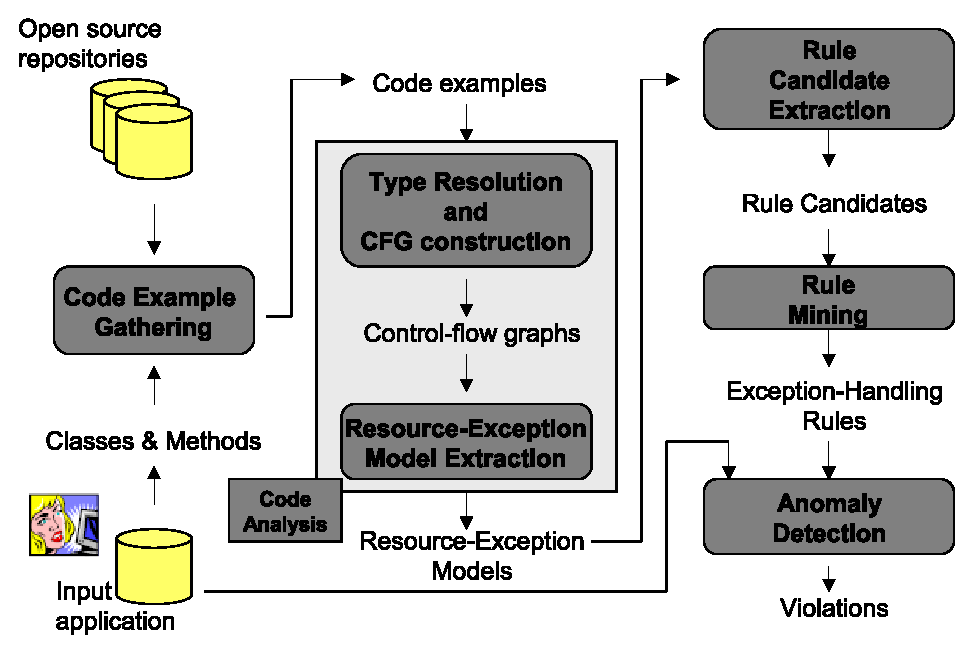
\includegraphics[scale=0.75,clip]{figs/architecture1.eps}\vspace*{-1ex}
\caption{Overview of our $\smoot$ approach.} \label{fig:architecture}
\vspace*{-3ex}
\end{figure*}

Figure~\ref{fig:architecture} shows a high-level overview of our $\smoot$ approach. $\smoot$ accepts an application under test and identifies classes and interfaces, declared or used by the application under test. These applications under test can also be frameworks or libraries. We refer to extracted classes for which sequences need to be collected as target classes, denoted by \{$TC_1$, $TC_2$, ..., $TC_m$\}. $\smoot$ also accepts a set of existing code bases, denoted by \{$CB_1$, $CB_2$, ..., $CB_n$\}, that already use these target classes. In our prototype implemented for the $\smoot$ approach, these code bases are in the form of .NET assemblies. Initially, $\smoot$ searches for relevant method bodies by using target classes as keywords. $\smoot$ constructs control-flow graphs for these method bodies and extracts sequences that produce objects of target classes. $\smoot$ extracts sequences by traversing these control-flow graphs. These extracted  sequences are used to assist random and DSE-based approaches. For DSE-based approaches, $\smoot$ converts extracted sequences into skeletons by replacing constant values for primitive types with symbolic values. We next explain each phase of MSeqGen in detail using the illustrative example shown in Figure~\ref{fig:mut}.

\begin{figure}[t]
\begin{CodeOut}
\begin{alltt}
00:public void Sort(VertexAndEdgeProvider vo) \{
01:\hspace*{0.1in}AdjacencyGraph g = new AdjacencyGraph(vo, true);
02:\hspace*{0.1in}Hashtable iv = new Hashtable();			
03:\hspace*{0.1in}int i = 0;  //adding vertices
04:\hspace*{0.1in}IVertex a = g.AddVertex();
05:\hspace*{0.1in}iv.Add(a);
06:\hspace*{0.1in}IVertex b = g.AddVertex();
07:\hspace*{0.1in}iv.Add(b);
08:\hspace*{0.1in}IVertex c = g.AddVertex();
09:\hspace*{0.1in}iv.Add(c);
10:\hspace*{0.1in}g.AddEdge(a,b);	//adding edges
11:\hspace*{0.1in}g.AddEdge(a,c);
12:\hspace*{0.1in}g.AddEdge(b,c);
13:\hspace*{0.1in}//TSAlgorithm: TopologicalSortAlgorithm
14:\hspace*{0.1in}TSAlgorithm topo = new TSAlgorithm(g);
15:\hspace*{0.1in}topo.Compute(); ... \}
\end{alltt}
\end{CodeOut}\vspace*{-4ex}
\Caption{\label{fig:adjacencyEx} A relevant method body for classes \CodeIn{AdjacencyGraph}, \CodeIn{VertexAndEdgeProvider}, \CodeIn{Hashtable}, and \CodeIn{TopologicalSortAlgorithm}.}\vspace*{-4ex}
\end{figure}

%-------------------------------------------------------------------------------
\subsection{Code Searching} 

We use code searching in our approach since code bases are often large and analyzing complete code bases can be prohibitively expensive. To avoid analyzing complete code bases, we use a keyword search to identify relevant method bodies including target classes. In particular, we use a text-based search, where the text is derived by decompiling .NET assemblies taken as inputs. We consider that a method body is relevant to a target class $TC_j$, if the method body includes the name of the $TC_j$ target class. For example, we use \CodeIn{AdjacencyGraph} as a keyword and search for method bodies including that keyword. Figure~\ref{fig:adjacencyEx} shows an example method body including the \CodeIn{AdjacencyGraph} keyword. As our code search is primarily a text-based search, code searching also returns irrelevant method bodies such as method bodies that include \CodeIn{AdjacencyGraph} as a variable name or a word in comments. We filter out such irrelevant method bodies in subsequent phases. 

We use intra-procedural analysis to analyze only such relevant method bodies. We use intra-procedural analysis since intra-procedural analysis is more scalable than inter-procedural analysis. Although intra-procedural analysis is less precise than inter-procedural analysis, we address this precision issue by using an iterative strategy explained in subsequent sections. 

%TODO : Add more arguments of why we used intra-procedural analysis.

%-------------------------------------------------------------------------------
\subsection{Code Analysis} 

We next analyze each relevant method body statically and construct a control-flow graph (CFG). Our CFG includes four
types of statements: method calls, object creations, typecasts, and field accesses. The rationale behind choosing these statements is that these statements result in generating objects of target classes. While constructing a CFG, we identify the nodes (in the constructed CFG) that produce the target classes such as \CodeIn{AdjacencyGraph} and mark them as \emph{nodes of interest}. For example, the node corresponding to Statement 1 in Figure~\ref{fig:adjacencyEx} is marked as a node of interest for the target class \CodeIn{AdjacencyGraph}. We also filter out irrelevant method bodies identified during the code searching phase if their related CFGs do not contain any nodes of interest.

We next extract sequences from a CFG using nodes of interest. For each node of interest related to a target class $TC_j$, we gather a path from the node of interest to the end of the CFG. In the case of loops, we consider the nodes inside a loop as a group of nodes that is executed either once or not. Considering these nodes once can help identify the sequence inside the loop. We also annotate these nodes to store the additional information that these nodes (and their associated method calls) exist inside loops. This additional information is used in subsequent phases while generating code based on extracted sequences.

Often, an extracted sequence can include a few method calls that are unrelated to the target class $TC_j$. We use data-dependency analysis to filter out such unrelated method calls from the extracted sequence. We start with the method call (in short as \emph{base method call}) associated with a node of interest and filter out method calls that do not share the same receiver object as the base method call. Our data-dependency analysis results in a sequence that creates and mutates an object of a target class $TC_j$. For example, Figure~\ref{fig:agraphseq} shows a sequence gathered from the code example in Figure~\ref{fig:adjacencyEx}. $\smoot$ extracts several such  sequences for different classes from the same code example. For example, if the set of target classes also includes classes \CodeIn{Hashtable} and \CodeIn{TSAlgorithm}, $\smoot$ automatically extracts one  sequence for each of these classes as shown below from the code example. 

\begin{CodeOut}
\begin{alltt}
\emph{Sequence for Hashtable}:
\hspace*{0.3in}IVertex a,b,c; //requires as input
\hspace*{0.3in}Hashtable iv = new Hashtable();
\hspace*{0.3in}iv.Add(a);
\hspace*{0.3in}iv.Add(b);
\hspace*{0.3in}iv.Add(c);

\emph{Sequence for TSAlgorithm}:
\hspace*{0.3in}AdjacencyGraph g; //requires as input
\hspace*{0.3in}TSAlgorithm tsObj = new TSAlgorithm(g);
\hspace*{0.3in}tsObj.compute();
\end{alltt}
\end{CodeOut}

%\textbf{Handling new non-primitive types.} 
One issue with extracted sequences is that these sequences can include additional non-primitive types. For example, the  sequence for \CodeIn{AdjacencyGraph} (shown in Figure~\ref{fig:agraphseq}) requires non-primitive type \CodeIn{VertexAndEdgeProvider}. To achieve target states, we need new sequences for generating these additional non-primitive types. In principle, call sites in code bases including sequences for a $TC_j$ target class also include sequences for generating related additional non-primitive types. However, in practice, often these call sites do not include sequences for these additional non-primitive types due to two factors. (1) A sequence for an additional non-primitive type is available in another method body and is not found by our approach as it uses intra-procedural analysis for extracting sequences.  (2) A sequence for an additional non-primitive type does not exist in the current code base $CB_i$ (such as a framework or a library) and expects a reusing application to provide a necessary sequence. 

We address this issue by extracting new sequences for additional non-primitive types by using an iterative strategy. More specifically, we first extract sequences for the initial set of target classes and collect all additional classes for which new sequences need to be extracted. We next extract sequences for these additional classes and collect more new additional classes. We repeat this process either till no new additional classes are collected or we reach a fixed number of iterations accepted as a configuration parameter, denoted by \emph{NUM\_ITERATIONS}. A high value for \emph{NUM\_ITERATIONS} can help collect more sequences; however, a high value can require more time for collecting those sequences. In our approach, we use five as the value of \emph{NUM\_ITERATIONS}, which is set based on our initial empirical experience.

%-----------------------------------------------------------------------
\subsection{Method-Call Sequence Generalization}

\begin{figure}[t]
\begin{CodeOut}
\begin{alltt}

\emph{A. Class Definition}:
00:class MyClass \{ 
01:\hspace*{0.1in}private int testMe;	
02:\hspace*{0.1in}private String ipAddr;	
03:\}

\emph{B. MUT}:
00:public void Mut1(MyClass mc, String IPAddress) \{
01:\hspace*{0.1in}if(mc.getTestMe() > 100) \{ 
02:\hspace*{0.2in}if(IsAValidIPAddress(IPAddress)) \{ ... \}
03:\hspace*{0.1in}\}
04:\}

\emph{C. Method-call sequence (MCS)}:
00:MyClass mcObj = new MyClass();
01:mcObj.SetTestMe(10);
02:mcObj.SetIpAddr("127.0.0.1");

\emph{D. Skeleton}:
00:int symvar = *, string ipaddr = *; 
01:MyClass mcObj = new MyClass();
02:mcObj.SetTestMe(symvar);
03:mcObj.SetIpAddr(ipaddr);

\end{alltt}
\end{CodeOut}\vspace*{-5ex}
\Caption{\label{fig:seqgeneralization} An illustrative example for method-call sequence generalization.}\vspace*{-3ex}
\end{figure}

%\emph{E. Skeleton with a boolean switch}:
%00:int symvar = *, string ipaddr = *; boolean bSymSwitch = *;
%01:if(bSymSwitch) \{
%02:\hspace*{0.1in}MyClass mcObj = new MyClass();
%03:\hspace*{0.1in}mcObj.SetTestMe(symvar);
%04:\hspace*{0.1in}mcObj.SetIpAddr(ipaddr);
%05:\} else \{
%06:\hspace*{0.1in}MyClass mcObj = new MyClass();
%07:\hspace*{0.1in}mcObj.SetTestMe(10);
%08:\hspace*{0.1in}mcObj.SetIpAddr("127.0.0.1");
%09:\}

We generalize sequences to address an issue that constant values in extracted sequences can be different from values required to achieve target states. We refer to the process of converting sequences into skeletons (which are sequences with symbolic values instead of concrete values for primitive types) as \emph{sequence generalization}. For example, consider a simple MUT and an example sequence (denoted as MCS) shown in Figures~\ref{fig:seqgeneralization}a to \ref{fig:seqgeneralization}c, respectively. The sequence cannot directly achieve the \CodeIn{true} branch of the MUT since the value of \CodeIn{testMe} is set to 10. To address this issue, we generalize extracted sequences. More specifically, we replace constant values of primitive types in extracted sequences with symbolic values. Figure~\ref{fig:seqgeneralization}d also shows the skeleton, where a symbolic variable \CodeIn{symvar} of type \CodeIn{int} is taken as input for the sequence. This \CodeIn{symvar} variable replaces the constant value 10 in the MCS. When this skeleton is used along with a DSE-based approach, the DSE-based approach initially generates a concrete random value for the \CodeIn{symvar} symbolic variable and gathers the constraint ($>$ $100$) in the MUT through dynamic execution. The DSE-based approach next solves the constraint to generate another concrete value for \CodeIn{symvar} such as $200$ that satisfies the gathered constraint. 

Although DSE-based approaches are effective in practice, it is challenging for these approaches to generate concrete values for variables that require complex values such as doubles, IP addresses, or URLs. In such cases, constant values in extracted sequences are useful in quickly covering those related branches such as the \CodeIn{true} branch in Statement 2 (Figure~\ref{fig:seqgeneralization}b) of the MUT. To address this issue, we preserve constant values in sequences along with the newly introduced symbolic values by using a symbolic \CodeIn{boolean} value as a switch between symbolic and constant values.
%TODO: Put a component called CodeGenerator. Show how we generate code automatically for Randoop and Pex. Also show how we handle loops.
%-----------------------------------------------------------------------
\subsection{Generation of New Sequences}

$\smoot$ extracts sequences from code bases and uses these sequences to assist random and DSE-based approaches. However, in some cases, these extracted sequences individually are not sufficient to achieve target states. $\smoot$ tries to address this issue by generating new sequences from extracted sequences by combining extracted sequences randomly. For example, consider two target classes $T_i$ and $T_j$, where $T_j$ requires an object of $T_i$ and a MUT requires an object of $T_j$. Consider that $\smoot$ identified two method bodies, denoted by $MD_1$ and $MD_2$, in code bases relevant to both $T_i$ and $T_j$. Consider that $\smoot$ extracted sequences $S_i^1$ and $S_j^1$ for target classes $T_i$ and $T_j$ from $MD_1$, respectively. Similarly, $\smoot$ extracted sequences $S_i^2$ and $S_j^2$ for target classes $T_i$ and $T_j$ from $MD_2$, respectively. The target class $T_i$ has sequences $S_i^1$ and $S_i^2$, and the target class $T_j$ has sequences $S_j^1$ and $S_j^2$. Given these sequences, $\smoot$ can generate some or all of four different combinations of these sequences for generating objects of $T_j$. These new sequences may further help achieve target states in the MUT.

\Comment{
For example, consider the following code example that includes two method bodies relevant to target classes \CodeIn{A} and \CodeIn{B}.

\begin{CodeOut}
\begin{alltt}
public void t1() \{
\hspace*{0.3in}A aobj = new A();
\hspace*{0.3in}aobj.ma1();
\hspace*{0.3in}B bobj = new B(aobj);
\hspace*{0.3in}bobj.mb1();
\}

public void t2() \{
\hspace*{0.3in}A aobj = new A();
\hspace*{0.3in}aobj.ma2();
\hspace*{0.3in}B bobj = new B(aobj);
\hspace*{0.3in}bobj.mb2();
\}
\end{alltt}
\end{CodeOut}

$\smoot$ extracts two  sequences each for classes \CodeIn{A} and \CodeIn{B} from the preceding code example. Extracting such individual  sequences can help generate new sequences such as a sequence including method calls \CodeIn{A.ma1} and \CodeIn{B.mb2}. These new sequences cannot be computed when long sequences with multiple classes are extracted. Our approach computes these combinations randomly.}

\section{Evaluation}
\label{sec:eval}

We conducted three different evaluations to show the effectiveness of our $\smoot$ approach. In our evaluations, we used two popular .NET applications: QuickGraph~\cite{QUICKGRAPH} and Facebook~\cite{FACEBOOK}. Our empirical results show that $\smoot$ handles large code bases and extracts sequences that can help achieve target states. Our empirical results also show that our approach can effectively assist random and DSE-based approaches in achieving higher branch coverage. The details of subjects and results of our evaluation are available at \url{http://research.csc.ncsu.edu/ase/projects/mseqgen/}. \\ All experiments were conducted on a machine with 1.6GHz Xeon processor and 1GB RAM. We next present research questions addressed in our evaluations.

%------------------------------------------------------------------------
\subsection{Research Questions}

In our evaluations, we address the following research questions.\vspace*{-1ex}

\begin{itemize}
\item RQ1: Can our approach handle large code bases in gathering sequences for target classes of subject applications?
\item RQ2: Can our approach assist a random approach in achieving higher code coverage of the code under test than without the assistance of our approach?
\item RQ3: Can our approach assist a DSE-based approach in achieving higher code coverage of the code under test than without the assistance of our approach?
\end{itemize}

%------------------------------------------------------------------------
\subsection{Subject Applications}

We used two popular .NET applications for evaluating our $\smoot$ approach: QuickGraph~\cite{QUICKGRAPH} and Facebook~\cite{FACEBOOK}. QuickGraph is a C\# graph library that provides various directed/undirected graph data structures. QuickGraph also provides algorithms such as depth-first search, breadth-first search, and A* search~\cite{thomas:algos}. 
QuickGraph includes 165 classes and interfaces with 5 KLOC. Facebook is a popular social network website that connects people with friends and others whom they work, study, and live around. In our evaluation, we use a Facebook developer toolkit that provides APIs necessary for developing Facebook applications. The Facebook developer toolkit includes 285 classes and interfaces with 40 KLOC.

%------------------------------------------------------------------------
\subsection{RQ1: Gathering Sequences}

We next address the first research question on whether our approach can handle large code bases in gathering sequences for target classes of the QuickGraph and Facebook applications. For QuickGraph and Facebook, we use code bases including 3.85 MB and 5 MB of .NET assembly code, respectively. Our approach extracted 167 sequences for QuickGraph with a maximum length of 12 method calls for the \CodeIn{AdjacencyGraph} class. Our approach took 5.2 minutes for analyzing code bases related to QuickGraph. For Facebook, our approach extracted 355 sequences with a maximum length of 51 method calls for the \CodeIn{Hashtable} class.  Although the sequence extracted for \CodeIn{Hashtable} is long, this sequence includes method calls such as \CodeIn{Add} for multiple times. Our approach took 4.5 minutes for analyzing code bases related to Facebook and to gather these sequences. Our results show that our approach can mine large code bases for gathering sequences to help achieve target states.

%------------------------------------------------------------------------
\subsection{RQ2: Assisting Random Approach}

We next address the second research question on whether our approach helps increase branch coverage achieved by a state-of-the-art random approach, called Randoop~\cite{pacheco:feedback}. To address this research question, we first run Randoop on QuickGraph and Facebook applications, and generate test inputs. Randoop generates test inputs in the form of sequences of method calls. We execute generated test inputs and measure branch coverage using a coverage measurement tool, called NCover\footnote{\url{http://www.ncover.com/}}. This measured coverage forms a baseline for comparing Randoop with and without the assistance from our approach. In our evaluation, we use default configurations provided by the Randoop developers. For each namespace of the subject application, we ran Randoop for a maximum of 130 seconds.

To assist Randoop with our extracted sequences, we synthesize static method bodies that include our gathered sequences and return objects of target classes of our subject applications. For example, if a target class $TC_j$ has four sequences, we synthesize four static method bodies where each method body returns an object of $TC_j$ by executing a gathered sequence for $TC_j$. If a sequence for $TC_j$ requires other objects of non-primitive or primitive types (whose values are not known in gathered sequences due to static analysis), we add those non-primitive and primitive types as arguments for the method bodies. For primitive types, Randoop randomly generates some values. For non-primitive types, Randoop randomly generates a new sequence or selects some other method body (synthesized by our approach) that produces that non-primitive type. We gather newly generated test inputs that include the method bodies synthesized by $\smoot$ and add these new test inputs to existing tests to measure the increase in the branch coverage. 

\setlength{\tabcolsep}{1pt}
\begin{table*}[t]
\begin{SmallOut}
\begin{CodeOut}
\begin{center}
\begin {tabular} {|l|c|c|c|c|c|}
\hline
\textbf{Application} & \textbf{\#} of & \textbf{Test Code} & \textbf{Random} & \textbf{Random + $\smoot$} & \textbf{\% Increase in }\\
 & \textbf{classes} & \textbf{T} & \textbf{R} & \textbf{R + M} & \textbf{Branch coverage}\\
\hline
\hline QuickGraph.Algorithms & 104 & 18.4 & 63.3 & 63.3 & - \\
\hline QuickGraph.Algorithms.Search & 11 & 40.3 & 33.3 & 47.6 & \textbf{14.3} \\
\hline QuickGraph.Algorithms.ShortestPath & 4 & 0 & 29.3 & 30.2 & 0.9 \\
\hline QuickGraph.Algorithms.Visitors & 11 & 0 & 86.4 & 86.4 & - \\
\hline QuickGraph.Collections & 19 & 11.2 & 74.0 & 83.3 & 9.3 \\
\hline QuickGraph.Exceptions & 3 & 40.0 & 100.0 & 100.0 & - \\
\hline QuickGraph.Predicates & 9 & 8.6 & 43.1 & 48.3 & 5.2 \\
\hline QuickGraph.Providers & 1 & 100.0 & 80.0 & 100.0 & \textbf{20.0} \\
\hline QuickGraph.Representations & 3 & 43.1 & 35.1 & 49.0 & \textbf{13.9} \\
\hline facebook & 25 & 48.9 & 14.0 & 23.3 & 9.3 \\
\hline facebook.Components & 3 & 0 & 30.7 & 30.7 & - \\
\hline facebook.desktop & 14 & 0 & 18.5 & 21.0 & 2.5 \\
\hline facebook.Forms & 4 & 0 & 11.1 & 11.1 & - \\
\hline facebook.Properties & 1 & 31.3 & 37.5 & 37.5 & - \\
\hline facebook.Schema & 216 & 6.1 & 20.8 & 24.8 & 4.1 \\
\hline facebook.Types & 1 & 0 & 100.0 & 100.0 & - \\
\hline facebook.Utility & 8 & 49.1 & 22.6 & 37.7 & \textbf{15.1} \\
\hline facebook.web & 12 & 0 & 3.3 & 4.5 & 1.2 \\
%\hline \textbf{AVERAGE} &  & 22 & 44.61 & 49.92 &  \\
\hline \textbf{AVERAGE} &  &  &  &  & \textbf{8.7} \\
\hline
\end{tabular}
\end{center}
\end{CodeOut}
\end{SmallOut}\vspace*{-4ex}
\centering \caption {\label{tab:premresults} Evaluation results showing higher branch coverage achieved by Randoop with the assistance of $\smoot$. \CodeIn{T: Test code, R: Randoop, M: $\smoot$}}
\end{table*}

Table~\ref{tab:premresults} shows the results of our evaluation with both subject applications. The table shows the results for all namespaces of the subject applications. As we include test code available with subject applications in code bases used for extracting sequences, we show branch coverage achieved by the test code alone in Column ``T''. Column ``R'' shows branch coverage achieved by Randoop. Column ``R + M'' shows branch coverage achieved by Randoop with the assistance of our $\smoot$ approach. Column ``Increase in Branch Coverage'' shows additional branch coverage achieved with the assistance from our $\smoot$ approach. As shown in our results, ``R + M'' achieved higher coverage than Randoop and test code (except for namespaces \CodeIn{facebook} and \CodeIn{facebook.Utility}). There are two primary reasons for lower coverage of ``R + M'' for these two namespaces: the random mechanism of Randoop and limitations of our current implementation. Due to the random mechanism used by Randoop, various method calls used in test code that contributed to higher coverage achieved by the test code are not used by Randoop in generating test inputs. Section~\ref{sec:future} presents limitations of our current implementation on why ``R + M'' achieved lower coverage than existing test code for namespaces \CodeIn{facebook} and \CodeIn{facebook.Utility}. Our results show that there is a considerable increase of 8.7\% on average\footnote{We compute average from those namespaces that have a non-zero increase in the branch coverage} (with a maximum of 20\%) in branch coverage achieved by Randoop with assistance from our approach. 

\begin{figure}[t]
\begin{CodeOut}
\begin{alltt}
00:class BidirectionalGraph \{ ...
01:\hspace*{0.1in}public IEdge AddEdge(IVertex src, IVertex tg) \{
02:\hspace*{0.2in}// look for the vertex in the list
03:\hspace*{0.2in}if (!VertexInEdges.ContainsKey(src))
04:\hspace*{0.3in}throw new VertexNotFoundException 
\hspace*{0.5in}("Could not find source");
05:\hspace*{0.2in}if (!VertexInEdges.ContainsKey(tg))
06:\hspace*{0.3in}throw new VertexNotFoundException 
\hspace*{0.5in}("Could not find target");
07:\hspace*{0.2in}// create edge
08:\hspace*{0.2in}IEdge e = base.AddEdge(src, tg);
09:\hspace*{0.2in}VertexInEdges[target].Add(e);
10:\hspace*{0.2in}return e;
11:\hspace*{0.1in}\}
12:\}
\end{alltt}
\end{CodeOut} \vspace*{-5ex}
\Caption{\label{fig:vidMUT} A MUT \CodeIn{AddEdge} in the \CodeIn{BidirectionalGraph} class of QuickGraph.} \vspace*{-5ex}
\end{figure}

We next provide examples to describe scenarios where our approach can assist random approaches. We also describe scenarios where our approach cannot assist random approaches. We use a MUT, called \CodeIn{AddEdge}, in the \CodeIn{BidirectionalGraph} class of the \CodeIn{QuickGraph.Representations} namespace (shown in Figure~\ref{fig:vidMUT}). Although Randoop generated three test inputs (in the form of sequences) for the \CodeIn{AddEdge} MUT, Randoop achieved low branch coverage of 40.0\% (2 out of 5 branches). The reason for not achieving high coverage for the \CodeIn{AddEdge} MUT is that the \CodeIn{AddEdge} MUT requires a specific receiver object state. To reach Statement 8 of the MUT, the \CodeIn{VertexInEdges} field should include the new vertices represented by \CodeIn{src} and \CodeIn{tg} that are passed as arguments. With the sequences extracted by our approach, Randoop achieved a branch coverage of 80.0\% (4 out of 5 branches). As our sequences are extracted from code bases that include usage scenarios on how these method calls are used in real practice, our sequences helped achieve high coverage for the \CodeIn{AddEdge} MUT. 

Although Randoop achieved higher branch coverage with the assistance from our approach, the test inputs generated by Randoop did not cover the \CodeIn{true} branch of Statement 5 to reach Statement 6. The reason is that our sequences do not include a usage scenario where the \CodeIn{AddEdge} MUT is invoked with one vertex in \CodeIn{VertexInEdges} and the other vertex not in \CodeIn{VertexInEdges}. Such usage scenarios rarely exist in code bases that are used for extracting sequences as these usage scenarios are related to testing the MUT for negative cases rather than reusing the MUT in real practice. However, a more systematic approach such as a DSE-based approach can cover such not-covered branches with the assistance from our approach.

%------------------------------------------------------------------------
\subsection{RQ3: Assisting DSE-based Approaches}

We next address the third research question on whether our approach can help increase branch coverage achieved by a DSE-based approach. To address this research question, we use a state-of-the-art DSE-based approach called Pex~\cite{tillman:pexwhite}. Pex accepts PUTs as input and generates conventional unit tests from these PUTs using DSE. As PUTs are not available with our subject applications, we generated PUTs for each public method in our subject applications using the \emph{PexWizard} tool. PexWizard is a tool provided with Pex and this tool automatically generates PUTs for each public method in the application given as input. A PUT generated for the \CodeIn{Compute} MUT (Figure~\ref{fig:mut}) is shown below.

\begin{CodeOut}
\begin{alltt}
00:[PexMethod]
01:public void Compute01(
02:\hspace*{0.3in}[PexAssumeUnderTest]UndirectedDFS target,
03:\hspace*{0.3in}[PexAssumeUnderTest]Vertex s) \{
04:\hspace*{0.1in}target.Compute(s);
05:\hspace*{0.1in}Assert.Inconclusive("this test has to be reviewed");
06:\}
\end{alltt}
\end{CodeOut}

The receiver object and argument objects required for the \CodeIn{Compute} MUT are accepted as arguments for the PUT. Pex generates skeletons for the non-primitive arguments by using a heuristic-based approach (Section~\ref{sec:pex}). For this evaluation, we used only the QuickGraph application. The reason is that Pex does not terminate in generating unit tests for the Facebook application. In future work, we plan to investigate the issues with Pex and apply Pex on the Facebook application. To provide a baseline for showing the effectiveness of our approach, we first applied Pex on PUTs generated for the QuickGraph application. We executed generated unit tests and measured branch coverage achieved by these unit tests for different namespaces in the QuickGraph application. In our evaluation, we use default configurations of Pex.

We next used our extracted sequences to assist Pex. Pex provides a feature called \emph{factory} methods, which allow programmers to provide assistance to Pex in generating non-primitive object types. We used this feature by converting our extracted sequences into factory methods. One issue with factory methods is that the current Pex allows only one factory method for a non-primitive object type. As our approach can extract multiple sequences for creating an object of a non-primitive type, we combine all sequences related to a non-primitive type into one factory method by using a \CodeIn{switch} statement. We next apply Pex on the subject application with new factory methods created based on our extracted sequences. We again generate unit tests using Pex and measure new branch coverage. 

\setlength{\tabcolsep}{1pt}
\begin{table}[t]
\begin{SmallOut}
\begin{CodeOut}
\begin{center}
\begin {tabular} {|l|c|c|c|c|}
\hline
\textbf{Application} & \textbf{\# C} & \textbf{P} & \textbf{P + M} & \textbf{Increase}\\
 &  &  &  & \textbf{\%}\\
\hline
\hline QuickGraph.Algorithms & 104 & 8.2 & 30.6 & \textbf{22.5}\\
\hline QuickGraph.Algorithms.Search & 11 & 0 & 13.9 & \textbf{13.9}\\
\hline QuickGraph.Algorithms.ShortestPath & 4 & 1.9 & 1.9 & -\\
\hline QuickGraph.Algorithms.Visitors & 11 & 50.0 & 50.0 & -\\
\hline QuickGraph.Collections & 19 & 14.9 & 29.0 & \textbf{14.1}\\
\hline QuickGraph.Exceptions & 3 & 60.0 & 60.0 & -\\
\hline QuickGraph.Predicates & 9 & 31.0 & 31.0 & -\\
\hline QuickGraph.Representations & 1 & 2.7 & 21.6 & \textbf{19.2}\\
\hline \textbf{AVERAGE} &  & & & \textbf{17.4}\\
\hline
\end{tabular}
\end{center}
\end{CodeOut}
\end{SmallOut}\vspace*{-4ex}
\centering \caption {\label{tab:pexresults} Evaluation results showing higher branch coverage achieved by Pex with the assistance of $\smoot$. \CodeIn{\# C: number of classes, P: Pex, M: $\smoot$}}\vspace*{-3ex}
\end{table}

Table~\ref{tab:pexresults} shows our results by applying Pex with and without our sequences on the QuickGraph application. On average, our approach helped increase the branch coverage by 17.4\% (with a maximum increase of 22.5\% for one namespace). Although there is a considerable increase in branch coverage with the assistance from our approach, overall Pex still achieved low branch coverage. This result is due to a limitation with the current Pex that cannot automatically identify implementing classes for interfaces and use their related factory methods. Often, factory methods created by our approach accept interfaces as arguments. Therefore, Pex is not able to identify relevant factory methods for interfaces, although factory methods for their implementing classes are created by our approach. In future work, we plan to address this limitation and we expect that our results can be much better after addressing this limitation of Pex.

We next present example scenarios where our approach is quite useful in achieving higher branch coverage with Pex. We use the  \CodeIn{TopologicalSortAlgorithm} class in the \CodeIn{QuickGraph.Algorithms} namespace as an illustrative example. Without the assistance from our approach, Pex did not achieve any coverage of the \CodeIn{TopologicalSortAlgorithm} class as Pex was not able to generate any sequences for creating objects of the \CodeIn{TopologicalSortAlgorithm} class. The reason for not able to generate any sequences is that the constructor of \CodeIn{TopologicalSortAlgorithm} accepts an interface as input. Using the factory methods generated by our approach, Pex achieved a branch coverage of 57.9\% (11 out of 19 branches). Our results show that our approach can assist DSE-based approaches in achieving higher code coverage than without using our approach.

\section{Threats to Validity}
\label{sec:threats}
The threats to external validity primarily include the degree to which the subject applications used in our evaluation are representative of true practice. We used two real non-trivial subjects in our evaluation: a medium-scale application QuickGraph~\cite{QUICKGRAPH} and a large-scale application Facebook~\cite{FACEBOOK}. These threats could be reduced by using more subjects in our evaluation. The threats to internal validity are instrumentation effects that can bias our results. Faults in our $\smoot$ prototype might cause such effects. Furthermore, faults in the tools for random and DSE-based approaches used in our evaluations might also cause such effects. To reduce these threats, we inspected a significant sample set of generated test results.

\section{Discussion and Future Work}
\label{sec:future}

Although random and DSE-based approaches show considerable increase in branch coverage with the assistance from our approach, overall coverage achieved by these approaches are still not close to 100\% coverage. The reason is that often code under test includes complex branches that are quite difficult to cover. We next give an example of a difficult branch that is not covered by any of the approaches used in our evaluation. We use the code example shown in Figure~\ref{fig:diffbranch} as an illustrative example. This difficult branch is in the \CodeIn{Visit} method of the \CodeIn{BreadthFirstSearchAlgorithm} class. The receiver-object state to reach Statement 8 requires that the \CodeIn{VisitedGraph} object has a non-empty set of vertices and edges. Reaching Statement 8 also requires a specific object state for the argument \CodeIn{s}. In particular, the vertex represented by the argument \CodeIn{s} should already exist in the \CodeIn{VisitedGraph} object and should have outgoing edges. Although our extracted sequences include a sequence for achieving a desirable receiver-object state, our sequences do not include a necessary sequence for achieving a desirable argument-object state. In future work, we plan to further address these issues by generating new sequences using evolutionary approaches~\cite{tonella:etoc,  inkumsah08:improving}. There, we can use our extracted sequences as an initial set for these evolutionary approaches to evolve. Generation of new sequences using evolutionary approaches can also help reduce the bias in our approach, where our approach gives more preference to verify common usage rather than uncommon usage.

\begin{figure}[t]
\begin{CodeOut}
\begin{alltt}
00:public void Visit(IVertex s) \{
01:\hspace*{0.1in}...
02:\hspace*{0.1in}m\_Q.Push(s);
03:\hspace*{0.1in}while (m\_Q.Count != 0) \{
04:\hspace*{0.2in}IVertex u = (IVertex)m\_Q.Peek(); 
05:\hspace*{0.2in}m\_Q.Pop();
06:\hspace*{0.2in}...
07:\hspace*{0.2in}foreach(IEdge e in VisitedGraph.OutEdges(u)) \{ 
08:\hspace*{0.3in}...		//Difficult branch
09:\hspace*{0.2in}\} 
10:\hspace*{0.1in}\}
11:\}
\end{alltt}
\end{CodeOut}\vspace*{-5ex}
\Caption{\label{fig:diffbranch} An example difficult branch not reached by any approach used in our evaluation.}\vspace*{-5ex}
\end{figure}

In our evaluations, for the \CodeIn{facebook} and \CodeIn{facebook.Utility} namespaces, branch coverage achieved by Randoop (with the assistance of our approach) is lower than branch coverage achieved by the test code (commonly written by  application developers). There are two primary reasons for lower coverage of these namespaces: limitations of the random mechanism of Randoop and our current implementation. Our current implementation does not handle several features such as inheritance or C\# generics. Therefore, our implementation could not capture some sequences due to their use of these features. In future work, we plan to extend our implementation to support these features. 

%In our current approach, gathering sequences is loosely coupled with dynamic symbolic execution. For example, we identify the target classes and gather method-call sequences from code bases. We next verify whether these sequences can help achieve the $\theta$ states. Therefore, some collected sequences can be irrelevant. In future work, we plan to identify a desirable target (such as a branch) that is not achieved by the dynamic symbolic execution and use that information to gather sequences. This additional information can help gather more relevant sequences. 

Our approach extracts sequences from code bases using the receiver or argument object types of a MUT (in a framework under analysis) and generates method bodies to assist test-generation approaches. Sometimes, these sequences may include object types specific to the code bases. For example, these object types can be classes that implement interfaces provided by the framework under analysis. In such scenarios, the method bodies generated by our approach are not compilable. Currently, we fix those compilation errors manually. In future work, we plan to automatically compile and verify extracted sequences to reduce this manual effort.

\Comment{We currently gather \emph{only} one path from a CFG to generate sequences. However, there can be different sequences
across multiple paths in the CFG. In future work, we plan to collect sequences from multiple paths in the CFG. We also plan to develop clustering heuristics to cluster similar sequences.}

Test-generation approaches~\cite{csallner:jcrasher, JTEST, pacheco:eclat, xie:rostra} were developed for object-oriented testing and these approaches accept a class under test (CUT) and generate random sequences of method calls belonging to the CUT with random values for method arguments. Another set of approaches~\cite{inkumsah08:improving} replaces random values for method arguments with symbolic values and compute concrete values for these arguments by solving constraints inside the method under test. Tonella~\cite{tonella:etoc} proposed an approach that exploits genetic algorithms to generate new sequences evolved from an initial set of sequences. Tonella's approach requires the users to provide this initial set of sequences. Inkumsah and Xie~\cite{inkumsah08:improving} extended Tonella's approach by integrating evolutionary testing with symbolic execution. However, all these approaches cannot handle multiple classes and their methods due to a large search space of possible sequences. 

Randoop~\cite{pacheco:feedback} executes constructed sequences in each iteration and computes feedback in order to guide the search process to generate valid sequences. However, Randoop still relies on random techniques and cannot effectively generate sequences for achieving target states as shown in our evaluation. Our approach extracts sequences from code bases and use those sequences to assist other approaches such as Randoop in achieving higher structural coverage.

Our approach is also related to another category of approaches based on mining source code~\cite{Engler2001deviant, acharya06:mining, wasylkowski07:detecting, thummalapenta07:parseweb, thummalapenta09:mining}. These approaches mine code bases statically and extracts frequent patterns as implicit programming rules. These approaches use mining algorithms such as frequent itemset mining~\cite{wang:bide} or association rule mining~\cite{agarwal:association} for extracting frequent patterns. These mined programming rules are used for assisting programmers in writing code or detecting violations in an application under analysis. Our approach also uses static analysis for extracting patterns as sequences that can produce objects of receiver or arguments types of a MUT. Unlike these existing approaches, our approach uses extracted sequences in a novel way for assisting test-generation approaches in achieving high structural coverage.


Another category of existing work~\cite{Elbaum:capture, orso:capture, david:java} uses a capture-and-replay approach for generating unit tests. During the capture phase, their approach monitors the interaction of a unit such as the class under test with the rest of the system (to which the class belongs to). Their approach generates unit tests for the class under test based on monitored interactions. During the replay phase, their approach executes generated unit tests. Our previous approach, called UnitPlus~\cite{song07:unitplus}, captures sequences in existing test code and suggests those sequences to developers in reducing the effort of writing new unit tests. Our new $\smoot$ approach captures sequences from existing code bases but uses those sequences for assisting test-generation approaches. Unlike existing approaches that replay exactly the same captured behavior, our $\smoot$ approach replays beyond the captured behavior using techniques such as sequence generalization or generating new sequences by combining extracted sequences. 

\section{Conclusion}
\label{sec:concl}

Generation of desirable method-call sequences for achieving high structural coverage of the code under test is a known challenging problem in unit testing of object-oriented code. Existing work~\cite{csallner:jcrasher, khurshid:symbolic, xie:rostra} in addressing this problem is based primarily on the implementation information of the class under test. In this paper, we proposed the first approach that addresses this problem from a novel perspective of incorporating other sources of information such as how method calls are used in practice. Our approach gathers the information of how method calls are used in practice by mining code bases that use receiver or argument object types of a method under test. Our approach extracts sequences related to these object types and uses extracted sequences to enhance two state-of-the-art test-generation approaches: random testing and dynamic symbolic execution. We have demonstrated the effectiveness of our approach with  evaluations. Using sequences extracted by our approach, we showed that a random testing approach achieved 8.7\% (with a maximum of 20.0\% for one namespace) higher branch coverage and a DSE-based approach achieved 17.4\% (with a maximum of 22.5\% for one namespace) higher branch coverage than without using our approach. Such an improvement is significant since the branches that are not covered by these state-of-the-art approaches are generally quite difficult to cover. Our approach represents a step towards a new direction of leveraging research in the field of mining software engineering data to assist test generation, serving as a synergy between these two major research areas.

\section*{Acknowledgments}

We thank Shuvendu Lahiri and Thomas Ball for sharing Randoop used in our evaluations.

\bibliographystyle{abbrv}
\begin{thebibliography}{10}

\bibitem{acharya06:mining}
M.~Acharya, T.~Xie, and J.~Xu.
\newblock {Mining Interface Specifications for Generating Checkable Robustness
  Properties}.
\newblock In {\em Proc. ISSRE}, pages 311--320, 2006.

\bibitem{agarwal:association}
R.~Agrawal and R.~Srikant.
\newblock Fast algorithms for mining association rules in large databases.
\newblock In {\em Proc. VLDB}, pages 487--499, 1994.

\bibitem{Clarke:symbolic}
L.~Clarke.
\newblock {A System to Generate Test Data and Symbolically Execute Programs}.
\newblock {\em IEEE Trans. Softw. Eng.}, 2(3):215--222, 1976.

\bibitem{thomas:algos}
T.~H. Cormen, C.~Stein, R.~L. Rivest, and C.~E. Leiserson.
\newblock {\em Introduction to Algorithms}.
\newblock McGraw-Hill Higher Education, 2001.

\bibitem{csallner:jcrasher}
C.~Csallner and Y.~Smaragdakis.
\newblock {JC}rasher: an automatic robustness tester for {J}ava.
\newblock {\em Softw. Pract. Exper.}, 34(11):1025--1050, 2004.

\bibitem{random:duran}
J.~Duran and M.~Ntafos.
\newblock An evaluation of random testing.
\newblock {\em IEEE Trans. Softw. Eng.}, 10(4):438--444, 1984.

\bibitem{Elbaum:capture}
S.~Elbaum, H.~N. Chin, M.~B. Dwyer, and J.~Dokulil.
\newblock {Carving differential unit test cases from system test cases}.
\newblock In {\em Proc. FSE}, pages 253--264, 2006.

\bibitem{Engler2001deviant}
D.~Engler, D.~Y. Chen, S.~Hallem, A.~Chou, and B.~Chelf.
\newblock {Bugs as deviant behavior: a general approach to inferring errors in
  systems code}.
\newblock In {\em Proc. SOSP}, pages 57--72, 2001.

\bibitem{FACEBOOK}
Facebook developer toolkit, 2008.
\newblock \url{http://www.codeplex.com/FacebookToolkit}.

\bibitem{godefroid:dart}
P.~Godefroid, N.~Klarlund, and K.~Sen.
\newblock {DART}: {D}irected automated random testing.
\newblock In {\em Proc. PLDI}, pages 213--223, 2005.

\bibitem{inkumsah08:improving}
K.~Inkumsah and T.~Xie.
\newblock Improving structural testing of object-oriented programs via
  integrating evolutionary testing and symbolic execution.
\newblock In {\em Proc. ASE}, pages 297--306, 2008.

\bibitem{JTEST}
Parasoft. {J}test manuals version 5.1. {O}nline manual, 2006.
\newblock \url{http://www.parasoft.com}.

\bibitem{khurshid:symbolic}
S.~Khurshid, C.~S. Pasareanu, and W.~Visser.
\newblock {Generalized symbolic execution for model checking and testing}.
\newblock In {\em Proc. TACAS}, pages 553--568, 2003.

\bibitem{king:symex}
J.~C. King.
\newblock {Symbolic Execution and Program Testing}.
\newblock {\em Communications of the ACM}, 19(7):385--394, 1976.

\bibitem{koushik:cute}
S.~Koushik, M.~Darko, and A.~Gul.
\newblock {CUTE: a concolic unit testing engine for C}.
\newblock In {\em Proc. ESEC/FSE}, pages 263--272, 2005.

\bibitem{Xiyang:fitness}
X.~Liu, H.~Liu, B.~Wang, P.~Chen, and X.~Cai.
\newblock {A unified fitness function calculation rule for flag conditions to
  improve evolutionary testing}.
\newblock In {\em Proc. ASE}, pages 337--341, 2005.

\bibitem{orso:capture}
A.~Orso and B.~Kennedy.
\newblock {Selective capture and replay of program executions}.
\newblock {\em SIGSOFT Softw. Eng. Notes}, 30(4):1--7, 2005.

\bibitem{pacheco:eclat}
C.~Pacheco and M.~D. Ernst.
\newblock Eclat: Automatic generation and classification of test inputs.
\newblock In {\em Proc. ECOOP}, pages 504--527, 2005.

\bibitem{pacheco:feedback}
C.~Pacheco, S.~K. Lahiri, M.~D. Ernst, and T.~Ball.
\newblock Feedback-directed random test generation.
\newblock In {\em Proc. ICSE}, pages 75--84, 2007.

\bibitem{QUICKGRAPH}
{QuickGraph: A 100\% C\# graph library with Graphviz Support, Version 2.0},
  2008.
\newblock \url{http://www.codeproject.com/KB/miscctrl/quickgraph.aspx}.

\bibitem{david:java}
D.~Saff, S.~Artzi, J.~H. Perkins, and M.~D. Ernst.
\newblock {Automatic test factoring for Java}.
\newblock In {\em Proc. ASE}, pages 114--123, 2005.

\bibitem{song07:unitplus}
Y.~Song, S.~Thummalapenta, and T.~Xie.
\newblock {UnitPlus}: Assisting developer testing in eclipse.
\newblock In {\em Proc. ETX}, pages 26--30, 2007.

\bibitem{thummalapenta07:parseweb}
S.~Thummalapenta and T.~Xie.
\newblock {PARSEWeb}: A programmer assistant for reusing open source code on
  the web.
\newblock In {\em Proc. ASE}, pages 204--213, 2007.

\bibitem{thummalapenta09:mining}
S.~Thummalapenta and T.~Xie.
\newblock {M}ining exception-handling rules as sequence association rules.
\newblock In {\em Proc. ICSE}, pages 496--506, 2009.

\bibitem{tillman:pexwhite}
N.~Tillmann and J.~de~Halleux.
\newblock Pex white box test generation for .{NET}.
\newblock In {\em Proc. TAP}, pages 134--153, 2008.

\bibitem{tillmann05:parameterized}
N.~Tillmann and W.~Schulte.
\newblock {Parameterized Unit Tests}.
\newblock In {\em Proc. ESEC/FSE}, pages 253--262, 2005.

\bibitem{tonella:etoc}
P.~Tonella.
\newblock Evolutionary testing of classes.
\newblock In {\em Proc. ISSTA}, pages 119--128, 2004.

\bibitem{wang:bide}
J.~Wang and J.~Han.
\newblock {BIDE}: Efficient mining of frequent closed sequences.
\newblock In {\em Proc. ICDE}, pages 79 -- 88, 2004.

\bibitem{wasylkowski07:detecting}
A.~Wasylkowski, A.~Zeller, and C.~Lindig.
\newblock Detecting object usage anomalies.
\newblock In {\em Proc. ESEC/FSE}, pages 35--44, 2007.

\bibitem{xie:rostra}
T.~Xie, D.~Marinov, and D.~Notkin.
\newblock Rostra: A framework for detecting redundant object-oriented unit
  tests.
\newblock In {\em Proc. ASE}, pages 196--205, 2004.

\end{thebibliography}

\end{document}
